%-------------------
%-------------------
\chapter{Grundlagen}
%  Vergleich von Techniken, was gibt es alles, was wurde am Ende verwendet und warum

%--------------------------------
\section{Prozedurale Generierung}

Werden Inhalte, wie Texturen oder 3D-Objekte, generiert, ohne dass diese vor der Ausführung des Algorithmus festgelegt wurden, so wird dies als \emph{prozedurale Generierung} (PG) bezeichnet.
Ursprünglich wurde PG verwendet, weil der Speicherplatz auf Computern sehr begrenzt war. Große 3D-Landschaften oder andere vorgefertigte künstlerische Werke konnten nicht gespeichert werden.\\
Die Demoszene entstand in den 1980er Jahren und treibt PG ins Extreme. Sie zeigt mit künstlerischen Inhalten, dass beeindruckende Ergebnisse trotz stark limitiertem Speicherplatz möglich sind \bzw wie man das volle Potential von Computerhardware ausschöpft  \cite{DemoScene}. 

Auf heutigen Rechnern ist der Speicherplatz nicht mehr so begrenzt und es kann viel Inhalt für \zb PC-Spiele von Künstlern vorgefertigt werden. Trotzdem behält PG ihre Daseinsberechtigung, denn der Entwurf komplexer Inhalte, wie beispielsweise Landschaften mit viel Vegetation, ist aufwändig und benötigt viel Zeit. Hier können wieder Algorithmen aus der PG eingesetzt werden um Zeit und Arbeit zu sparen. Sie können sowohl verwendet werden um fertige 3D-Modelle zu generieren, als auch um als Inspiration und Hilfe für den Künstler zu dienen. \emph{SpeedTree} \cite{SpeedTree} ist ein Beispiel für Software, die für die Generierung von Vegetation verwendet wird. Sie unterstützt und beschleunigt die Erstellung von Szenen mit viel Vegetation. \cite{PCGSurvey_videoGames}

Dinge, die oft prozedural generiert werden, sind Landschaften, Straßennetze, Gebäude, Menschen, Tiere oder auch Geschichten \cite{PCGSurvey}. Humanoide Charaktere für Computerspiele werden \zb in der Masterarbeit \cite{ProceduralCharacterGeneration} erzeugt. Die Zusammenstellung \cite{PCGSurvey_videoGames} untersucht PG von Wesen, die Videospiele bevölkern. Obwohl einige Arbeiten genannt werden, die sich mit diesem Thema beschäftigen, wird auch festgestellt, dass dieser Themenbereich noch wenig erforscht ist. \\
Ein Beispiel, das erst nach Erscheinen dieser Zusammenstellung auf den Markt gekommen ist, ist das Computerspiel "`No Man's Sky"' \cite{NoMansSky}. Darin gibt es viele prozedural generierte fantastische Tiere. Die Generierung dieser Tiere funktioniert so, dass zunächst prozedural ein Modell generiert wird, in welches anschließend ein Skelett eingepasst wird \cite{NoMansSkyDevelopment}.
Die dort verwendeten Skelette sind nicht wirklichkeitsgetreu, sondern werden nur für die Animation verwendet (siehe Abschnitt \ref{character_animation}).

\todo{perlin noise (nicht ausreichend für Skelette, mehr Einschränkungen nötig sonst würden nur Monster generiert) + weitere Methodenbeispiele}


%--------------------------
\section{Inverse Kinematik}
\label{IK}

Inverse Kinematik wird unter anderem in der Robotik zur Bewegung von Robotern verwendet. Gegeben ist eine Kette von Gelenken, die über starre Verbindungsteile miteinander verbunden sind. Für ein oder mehrere Punkte dieser Kette können Zielpunkte im Raum angegeben werden. Das Ziel ist es dann eine Konfiguration der Gelenke zu berechnen, so dass alle Punkte ihr Ziel erreichen.\\
Es gibt viele verschiedene Methoden Probleme aus der inversen Kinematik zu lösen. Diese finden jeweils Abhängigkeit von der konkreten Problemstellung ihre Anwendung. Beispielsweise geht es in \cite{IKLegs} um die Animation von Beinen. Ein Überblick über die verschiedenen Techniken ist in Zusammenstellung \cite{IKSurvey} zu finden.

% IK die gelernte Posen bevorzugt: style-based inverse kinematics (\url{https://grail.cs.washington.edu/projects/styleik/})

%-------------------------------------------
\section{Charakteranimation}
\label{character_animation}

Um Charaktere für Computerspiele oder Filme zu animieren, ist außer dem 3D-Modell ein Skelett nötig. Dieses Skelett ist oft sehr abstrakt und hat wenig mit lebensechten Skeletten zu tun. Es gibt eine Baumstruktur auf den Einzelteilen des Charakters vor. Diese Baumstruktur ist für viele Algorithmen, die zur Animation verwendet werden essentiell, \zb für inverse Kinematik (siehe Abschnitt \ref{IK}). Als Wurzel für das Skelett wird ein Knochen nahe des Schwerpunkts des Charakters verwendet. Das ist bei humanoiden Charakteren die Hüfte.\\
Weit verbreitete Editoren für Animation, Modellierung, Simulation und Rendering sind Maya \cite{Maya} und 3ds Max \cite{3dsMax}. Auch hier werden solche Skelette verwendet \cite{MayaSkeletonHierarchy}. 3ds Max stellt \zb in einer Komponente namens Biped vorgefertigte Skelette für humanoide Charaktere zur Verfügung, die einfach in schon existierende 3D-Modelle eingefügt werden können \cite{3dsMaxBiped}.

Animationen werden dann mit Hilfe sogenannte Keyframes erzeugt. Keyframes sind Positionen, die der Charakter im Laufe der Bewegung einnehmen soll. Interpolation zwischen den einzelnen Keyframes ergibt dann eine flüssige Bewegung. \cite[Kapitel 3]{sporeanim}\\
Im Computerspiel Spore \cite{Spore} werden sogar zur Laufzeit Animationen für Charaktere erzeugt, deren Aufbau vorher noch nicht bekannt war. Dazu werden vorher abstrakte Animationen, unabhängig vom Aufbau des speziellen Charakters, erzeugt. Diese werden dann zur Laufzeit auf die konkreten Charaktere angewandt. \cite{sporeanim}

Um besonders lebensecht wirkende Tiere zu erzeugen, ist es nötig den Aufbau des entprechenden Tieres möglichst wirklichkeitsgetreu zu modellieren. Dazu sind Modelle für Skelett, Muskeln und Haut nötig. Solche Modelle lassen sich beispielsweise mit dem Maya-Plugin Ziva \cite{Ziva} erzeugen. \cite{ZivaGeneralSetup}

Der Algorithmus, der hier erarbeitet wird, erzeugt Skelette mit lebensechten Knochenmodellen. Er kann als Inspiration zur Erstellung neuer Charaktere dienen oder auch als Grundlage für ein Tier, das ein realitätsnahes Skelett haben soll.


% \begin{itemize}
%  \item Featherstone Algorithmus
%  \item skeleton-based design tool (Yamamoto et al 2011): rudimentäres Skelett/Rig für schnelle Produktion und leichte Änderung an Charakteren
%         \url{https://dl.acm.org/doi/10.1145/2073304.2073316}, \url{https://www.youtube.com/watch?v=yhq1aUp8QLY}
% \end{itemize}


%--------------------
\section{Grammatiken}
\label{grammars}

Eine \emph{Grammatik} ist ein Tupel $G = (\Sigma, N, S, P)$ mit 
\begin{itemize}
 \item dem endlichen Alphabet $\Sigma$ der Terminalsymbole
 \item dem endlichen Alphabet $N$ der Nichtterminalsymbole
 \item dem Startsymbol $S \in V$ und
 \item der Menge von Produktionen $P \subseteq (N \cup \Sigma)^* N (N \cup \Sigma)^* \times (N \cup \Sigma)^*$\\ der Form $P \subseteq (N \cup \Sigma)^* N (N \cup \Sigma)^* \rightarrow (N \cup \Sigma)^*$
\end{itemize}

Eine Teilmenge der Grammatiken bilden \emph{kontextsensitive} Grammatiken. Ihre Produktionen haben die Form
\[\alpha A \beta \rightarrow \alpha \gamma \beta \text{ oder } S \rightarrow \epsilon\] \[\text{ mit } A \in N,~ \alpha, \beta, \gamma \in ((N \setminus \{ S \}) \cup \Sigma)^*,~ \gamma \neq \epsilon \text{ und dem leeren Wort } \epsilon.\]

Wiederum eine Teilmenge davon bilden \emph{kontextfreie} Grammatiken mit Produktionen der Form 
\[A \rightarrow w \text{ mit } A \in N \text{ und } w \in (\Sigma \cup N)^*.\] \cite[Abschnitte 1.4 und 1.5]{FormalLanguageTheory}

\emph{L-Systeme} oder Lindenmayer-Systeme sind spezielle Grammatiken. Sie wurden 1968 von dem Biologen Aristid Lindenmayer vorgestellt, mit dem Zweck das Wachstum vielzelliger Lebewesen zu modellieren. Im Unterschied zu Grammatiken, bei denen Produktionen einzeln nacheinander angewendet werden, werden bei L-Systemen alle Symbole gleichzeitig ersetzt. Dies soll modellieren, dass viele Zellteilungen zur gleichen Zeit stattfinden können.\\
Es gibt auch hier wieder verschiedene Teilmengen wie \zb kontextfreie und kontextsensitive L-Systeme. Kontextfreie L-Systeme sind aber beispielsweise keine Teilmenge kontextfreier Grammatiken. Es gibt Sprachen, die von kontextfreien L-Systemen, aber nicht von kontextfreien Grammatiken erzeugt werden können und anders herum \cite[Abbildung 1.2]{AlgorithmicBeautyOfPlants}.\\
Oft werden L-Systeme verwendet um das Wachstum von Pflanzen zu modellieren. Es gibt aber auch andere Anwendungsbeispiele, wie \zb die Generierung von Städten \cite{cityGeneration}. 

Bei Pflanzen treten oft Verzweigungen auf. Um diese zu modellieren, werden Klammerstrukturen verwendet. Das Teilwort innerhalb einer Klammer repräsentiert einen "`Ast"', der wiederum in sich verzweigt sein kann.
Wenn zwei Symbole direkt aufeinander folgen, so bedeutet das, dass das linke Element das Elternelement des rechten ist. Kommt in einem Wort $A(BC)D$ mit $A, B, C, D \in \Sigma \cup N$ ein Klammerausdruck vor, so bedeutet dies, dass $A$ sowohl das Elternelement von $B$ als auch von $D$ ist. Das Elternelement von $C$ ist $B$. Es können auch Mehrfachverzweigungen auftreten. In $A(B)(C)D$, was gleichbedeutend ist zu $A(B)(C)(D)$, ist $A$ das Elternelement von $B, C$ und $D$. Eine Visualisierung der beiden Beispiele ist in Abbildung \ref{branching_examples} zu finden. \cite[Kapitel 1]{AlgorithmicBeautyOfPlants}

\begin{figure}
 \centering
 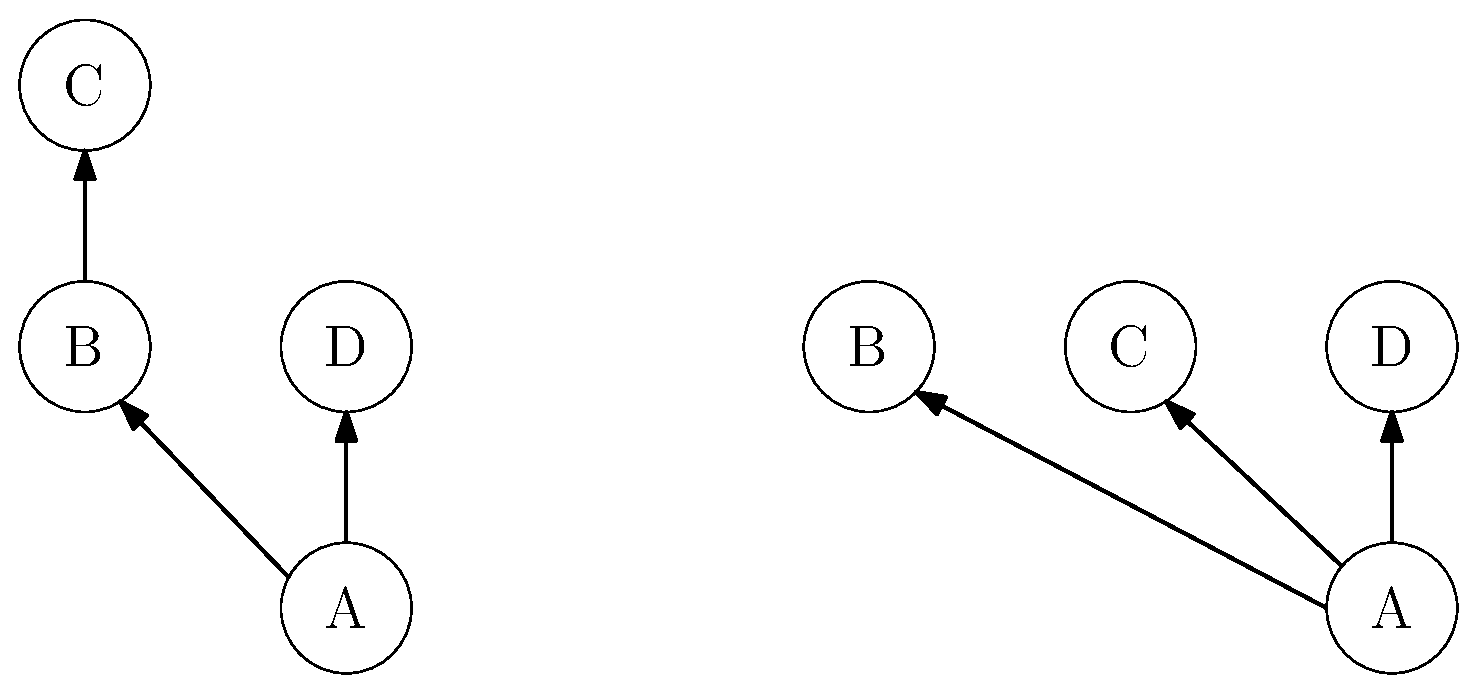
\includegraphics[width=0.6\textwidth]{graphics/branchingExamples}
 \caption{Visualisierung der Beispielklammerausdrücke,\\ links der \mbox{Ausdruck $A(BC)D$}, rechts $A(B)(C)D$.}
 \label{branching_examples}
\end{figure}


%------------
\section{PCA} % a priori algorithmus?
\label{PCA}
 
 % Ziel
 \emph{Principal Component Analysis} (PCA) oder auch Hauptkomponentenanalyse \cite{PCA} wird meist mit dem Ziel angewendet die Dimensionalität einer Menge von Datenpunkten zu verringern, dabei aber möglichst wenig Information zu verlieren.
 Beispielsweise wird dies in \cite{PCA_faces} bei 3D-Modellen von Gesichtern oder in \cite{PCA_bodies} bei 3D-Modellen von menschlichen Körpern gemacht. Auch im Zusammenhang mit prozeduraler Generierung wird PCA oft verwendet, \zb zur Generierung von humanoiden Charakteren für Videospiele \cite{ProceduralCharacterGeneration} oder Texturen für Gesichter \cite{GeneratingFacialTextures}.
 
 Als Ausgangspunkt für eine PCA dient eine Menge von Datenpunkten (oder Beispielen) $D$ im $n$-dimensionalen Raum. Voraussetzung ist, dass die Punkte in jeder Dimension normalverteilt sind. 
 Die Datenpunkte $D$ sind dann nach einer $n$-dimensionalen Normalverteilung verteilt. Betrachtet man nun die Wahrscheinlichkeitsdichte dieser Normalverteilung, so bilden alle Punkte, bei denen die Dichte einen Wert größer als $\epsilon$ annimmt das Innere eines $(n-1)$-dimensionalen Hyperellipsoids. In diesem Volumen liegen die meisten der Datenpunkte $D$. Den Mittelpunkt bildet ihr Mittelwert.
 
 Nun ist das Ziel herauszufinden wo die Achsen des Ellipsoids liegen. Betrachtet man die Komponenten der Datenpunkte $D$ in den Richtungen der Achsen, so sind diese wiederum normalverteilt und die Verteilungen sind jeweils unabhängig voneinander.
 Um die Achsen des Ellipsoids zu berechnen, wird zunächst die Kovarianzmatrix der Datenpunkte $D$ aufgestellt und dann diagonalisiert. In den Spalten der Basiswechselmatrix stehen dann die Eigenvektoren und auf der Diagonalen der diagonalisierten Kovarianzmatrix die Eigenwerte.
 Die Eigenvektoren sind die Achsen des Ellipsoids und die Eigenwerte geben die Varianz der Normalverteilung entlang der Achsen an.
 
 Jetzt können die Datenpunkte $D$ vom Eingabekoordinatensystem in dasjenige Koordinatensystem transformiert werden, das von den Achsen des Ellipsoids aufgespannt wird. Dazu stellt man die Punkte als Linearkombinationen der Eigenvektoren dar. 
 Um nun die Dimensionalität der Eingabedaten zu reduzieren, werden alle Dimensionen weggelassen, die nicht zu den Hauptkomponenten gehören. Je weniger Streuung die Datenpunkte auf denjenigen Achsen aufweisen, die weggelassen werden, desto weniger Information wird verworfen.
 
 Will man einen zufälligen Datenpunkt erzeugen, der die gleichen Verteilungen aufweist, wie die Eingabebeispiele, so funktioniert das im transformierten Koordinatensystem sehr gut. Da die einzelnen Dimensionen unabhängig voneinander sind, kann man einfach für jede Dimension eine normalverteilte Zufallszahl mit entsprechender Varianz generieren.
 
 
%---------------------------------- 
\section{Quantil-Quantil-Diagramme} 
\label{qqdiagrams}

Quantil-Quantil-Diagramme sind eine grafische Methode um zu testen, ob eine Stichprobe einer bestimmten Verteilung unterliegt. \\
Seien $x_1, x_2,\dots, x_n$ die Elemente einer Stichprobe und $F$ die Verteilungsfunktion derjenigen Verteilung, gegen die getestet werden soll. Die Verteilungsfunktion gibt für einen Wert $x$ an, wie groß die Wahrscheinlichkeit ist, dass die Zufallsvariable einen Wert $\leq x$ annimmt.\\
Nun werden die empirischen Quantile der Stichprobe mit den entsprechenden Quantilen von $F$ verglichen. Dazu wird die Stichprobe aufsteigend sortiert, was $x_{(1)}, x_{(2)},\dots, x_{(n)}$ ergibt. 
Das empirische $\frac{i}{n}$-Quantil der Stichprobe ist $x_{(i)}$, da $i$ Werte $\leq x_{(i)}$ beobachtet wurden. Die inverse Verteilungsfunktion gibt für einen Wert $y$ den kleinsten Wert $x$ an, für den gilt, dass $F(x) > y$, also das $y$-Quantil. Das $\frac{i}{n}$-Quantil von $F$ ist also $F^{-1}\left(\frac{i}{n}\right)$.

Trägt man nun die sortierte Stichprobe gegen die entsprechenden Quantile in ein Diagramm ab, und die angenommene Verteilung ist korrekt, so liegen die Punkte annähernd auf einer Geraden mit Steigung $1$ durch den Ursprung. \cite[Kapitel 1 und 2]{QQPlots}

Den Werten $x_{(i)}$ einfach das $\frac{i}{n}$-Quantil zuzuordnen ist aber insofern schwierig, als dass es suggeriert, dass alle Werte, die mit der angenommenen Verteilung generiert werden, kleiner als $x_{(n)}$ sind. Deshalb gibt es verschiedene andere Möglichkeiten die Quantile zuzuordnen. Sie liefern aber für $n \rightarrow \infty$ alle das gleiche Ergebnis. Sogenannte "`Rankit Plots"' verwenden folgende Zuordnung:
\[ x_{(i)} \approx F^{-1}\left(\frac{i - 0,5}{n}\right). \]
Diese Zuordnung wird auch in dieser Arbeit verwendet.


%-------------------------------
\section{Genetische Algorithmen}

als Alternative zu Variationen mit PCA

\begin{itemize}
 \item introduction to evolutionary design (bently)
 \item basics on genetic algorithms (Holland 1992) -> bei Bib bestellt
 \item interactive evolutionary computation (Takagi 2001) (fitness function = human evaluation)
 \item jon hudson thesis: creature generation using genetic algorithms \cite{JonHudson}
   \begin{itemize}
    \item relativ simple Regeln, nicht orientiert an spezieller Tierklasse, Einschränkung für Anzahl Beine, für Houdini, kein Skelett sondern 3D-Modell, Rig wird auch generiert
    \item auch Variationen eines Tiers und Crossover zwischen mehreren Exemplaren möglich
   \end{itemize}
  \item Grammar based genetic programming (a survey) 
\end{itemize}


